\documentclass[11pt]{article}
\usepackage{amsmath,amssymb,amsthm,bbm}
\usepackage{graphicx}
\usepackage{tikz,float}
\usepackage[colorlinks=true]{hyperref}
\DeclareMathOperator*{\E}{\mathbb{E}}
\DeclareMathOperator*{\sgn}{\mathrm{sign}}
\usepackage[ruled,noline]{algorithm2e}
\newcommand{\handout}[5]{
\noindent
\begin{center}
\framebox{
\vbox{
\hbox to 5.78in { {\bf CIS5200: Machine Learning } \hfill #2 }
\vspace{4mm}
\hbox to 5.78in { {\Large \hfill #5 \hfill} }
\vspace{2mm}
\hbox to 5.78in { {\em #3 \hfill #4} }
}
}
\end{center}
\vspace*{4mm}
}
\newcommand{\lecture}[5]{\handout{#1}{#2}{Release Date: #3}{Due Date: #4}{Homework
#1}}
\newtheorem{theorem}{Theorem}[subsection]
\newtheorem{corollary}[theorem]{Corollary}
\newtheorem{lemma}[theorem]{Lemma}
\newtheorem{observation}[theorem]{Observation}
\newtheorem{proposition}[theorem]{Proposition}
\newtheorem{definition}[theorem]{Definition}
\newtheorem{property}[theorem]{Property}
\newtheorem{claim}[theorem]{Claim}
\newtheorem{fact}[theorem]{Fact}
\newtheorem{assumption}[theorem]{Assumption}
\topmargin 0pt
\advance \topmargin by -\headheight
\advance \topmargin by -\headsep
\textheight 8.9in
\oddsidemargin 0pt
\evensidemargin \oddsidemargin
\marginparwidth 0.5in
\textwidth 6.5in
\parindent 0in
\parskip 1.5ex
\begin{document}
\lecture{4}{Spring 2025}{April 1, 2025}{April 15, 2025}
\noindent
\textbf{Name}: Haoze Wu \\
\textbf{PennKey}: haozewu \\
\textbf{Collaborators}: None
\subsection*{\Large Problem 1: AdaBoost}
\paragraph{1.1}
By definition, we have:
\begin{equation}
  \text{error}(H_T) := \frac{1}{m} \sum_{i=1}^m \mathbbm{1}[\text{sgn}(H_T(x_i)) \neq y_i] 
\end{equation}
To prove
\begin{equation}
  \text{error}(H_T) \leq \frac{1}{m} \sum_{i=1}^m \exp(-y_iH_T(x_i))
\end{equation}
is equivalent to prove that 
\begin{equation}
  \sum_{i=1}^m \mathbbm{1}[\text{sgn}(H_T(x_i)) \neq y_i] \leq \sum_{i=1}^m \exp(-y_iH_T(x_i))
\end{equation}
and noticing that for each data point $x_i$ in the dataset $X$, its error in the $T$-th iteration is given by the term:
\begin{equation}
  \mathbbm{1}[\text{sgn}(H_T(x_i)) \neq y_i] 
\end{equation}
When the prediction of the predictor in the $T$-th iteration is correct, this term is equal to 0, for the product of the prediction and correcponding label is given by:
\begin{equation}
  \begin{split}
  y_iH_T(x_i) &\leq 0 \\ 
  -y_iH_T(x_i) &\geq 0
  \end{split}
\end{equation}
and thus, the exponential term is :
\begin{equation}
  \begin{split}
  \exp(-y_iH_T(x_i)) &\geq 1 \\
  \mathbbm{1}[\text{sgn}(H_T(x_i)) \neq y_i] = 1 &\leq  \exp(-y_iH_T(x_i))
  \end{split}
\end{equation}
When the prediction of the predictor in the $T$-th iteration is incorrect, this term is equal to 1, for the product of the prediction and correcponding label is given by:
\begin{equation}
  \begin{split}
  y_iH_T(x_i) &\geq 0 \\ 
  -y_iH_T(x_i) &\leq 0
  \end{split}
\end{equation}
and thus, the exponential term is :
\begin{equation}
  \begin{split}
  0 < \exp(-y_iH_T(x_i)) &\leq 1 \\
  \mathbbm{1}[\text{sgn}(H_T(x_i)) \neq y_i] = 0 &<  \exp(-y_iH_T(x_i)) \leq 1
  \end{split}
\end{equation}
Thus, we have shown that for each data point $x_i$ in the dataset $X$, the following holds:
\begin{equation}
  \mathbbm{1}[\text{sgn}(H_T(x_i)) \neq y_i] \leq \exp(-y_iH_T(x_i))
\end{equation}
and thus, we can sum over all data points $x_i$ in the dataset $X$ to obtain:
\begin{equation}
  \sum_{i=1}^m \mathbbm{1}[\text{sgn}(H_T(x_i)) \neq y_i] \leq \sum_{i=1}^m \exp(-y_iH_T(x_i))
\end{equation}
and thus, we have shown that:
\begin{equation}
  \text{error}(H_T) \leq \frac{1}{m} \sum_{i=1}^m \exp(-y_iH_T(x_i))
\end{equation}
Proved.

\paragraph{1.2}
Noticing that the deifintion of the predictor in the $T$-th iteration is defined as:
\begin{equation}
  H_T(x) = \sum_{t=1}^T \alpha_t h_t(x)
\end{equation}
, then, by defintion, the weight $w_{t+1,i}$ is given by:
\begin{equation}
  w_{t+1, i} = \frac{w_{t,i}}{Z_t} \exp(-\alpha_t y_i h_t(x_i))
\end{equation}
, and thus using this recursive definition from $w_{1, i}$ to $w_{t+1, i}$, we have:
\begin{equation}
\begin{split}
 w_{t+1,i} &= \frac{w_{t,i}}{Z_t} \exp(-\alpha_t y_i h_t(x_i)) \\
&= \frac{w_{1,i}}{\prod_{t=1}^{T} Z_t} \prod_{t=1}^{T} \exp(-\alpha_t y_i h_t(x_i)) \\ 
&=\frac{1}{m\prod_{t=1}^{T} Z_t} \prod_{t=1}^{T} \exp(-\alpha_t y_i h_t(x_i)) \\
&= \frac{1}{m\prod_{t=1}^T Z_t}\exp(-y_iH_T(x_i))
\end{split}
\end{equation}
which indicates that:
\begin{equation}
  mw_{t+1,i} \prod_{t=1}^T Z_t= \exp(-y_iH_T(x_i))
\end{equation}
Then, we may sum all these terms over all data points $x_i$ in the dataset $X$ to obtain:
\begin{equation}
  \begin{split}
    \sum_{i=1}^m mw_{t+1,i} \prod_{t=1}^T Z_t &= \sum_{i=1}^m \exp(-y_iH_T(x_i))  \\
   m\sum_{i=1}^m w_{t+1,i} \prod_{t=1}^T Z_t &= \sum_{i=1}^m \exp(-y_iH_T(x_i))  \\
   m\prod_{t=1}^T Z_t &= \sum_{i=1}^m \exp(-y_iH_T(x_i))  \\
    \prod_{t=1}^T Z_t &= \frac{1}{m}\sum_{i=1}^m \exp(-y_iH_T(x_i))
  \end{split}
\end{equation}
, which is exactly the same as the equation given in the problem, which means that we proved that:
\begin{equation}
  \frac{1}{m}\sum_{i=1}^m \exp(-y_iH_T(x_i)) = \prod_{t=1}^T Z_t
\end{equation}

\paragraph{1.3}
From the definition of $Z_t$, we have:
\begin{equation}
  Z_t = \sum_{j=1}^m w_{t,j} \exp(-\alpha_t y_i h_t(x_j))
\end{equation}
We may categorize the data points into two groups, one group is correctly classified by the predictor and antoher is mistakenly classified by the predictor, and thus we have:
\begin{equation}
Z_t = \sum_{h_t(x_j) = y_j} w_{t,j} \exp(-\alpha_t y_i h_t(x_j)) + \sum_{h_t(x_j) \neq y_j} w_{t,j} \exp(-\alpha_t y_i h_t(x_j))
\end{equation}
By the definition of the weighted error, we then have:
\begin{equation}
\epsilon_t = \sum_{i=1}^m w_{t,i} \mathbbm{1}[h_t(x_i) \neq y_i] = \sum_{h_t(x_j) \neq y_j} w_{t,j}
\end{equation}
and the sum of weight of all the correctly classified data points is $1-\epsilon_t$, along with $y_ih_t(x_i)=1$ whet the data point $x_i$ is classfieid correctly abd $y_ih_t(x_i) = -1$ when it is wrong, and thus we have:
\begin{equation}
  Z_t = (1-\epsilon_t) \exp(-\alpha_t) + \epsilon_t \exp(\alpha_t)
\end{equation} 
Proved.

\paragraph{1.4}
From the statement proved in problem 1.3, we have:
\begin{equation}
  Z_t = (1-\epsilon_t) \exp(-\alpha_t) + \epsilon_t \exp(\alpha_t)
\end{equation}
To find the minized value of $Z_t$, we can take the derivative of $Z_t$ with respect to $\alpha_t$ and set it to 0:
\begin{equation}
  \begin{split}
    \frac{dZ_t}{d\alpha_t} &= -(1-\epsilon_t) \exp(-\alpha_t) + \epsilon_t \exp(\alpha_t) = 0 \\ 
    \epsilon_t \exp(\alpha_t) &= (1-\epsilon_t) \exp(-\alpha_t) \\
    \epsilon_t \exp(2\alpha_t) &= (1-\epsilon_t) \\
    \exp(2\alpha_t) &= \frac{1-\epsilon_t}{\epsilon_t} 
  \end{split}
\end{equation}
Taking the logarithm of both sides, we have:
\begin{equation}
  \alpha_t = \frac{1}{2}\log(\frac{1-\epsilon_t}{\epsilon_t})
\end{equation}
Proved.

\subsection*{\Large Problem 2: Auto-Differentiation}
\paragraph{2.1}
The following is the computation graph for the function $f(x,y) = x_1\cdot\ln(x_2)+x_1^2$:
\begin{center}
  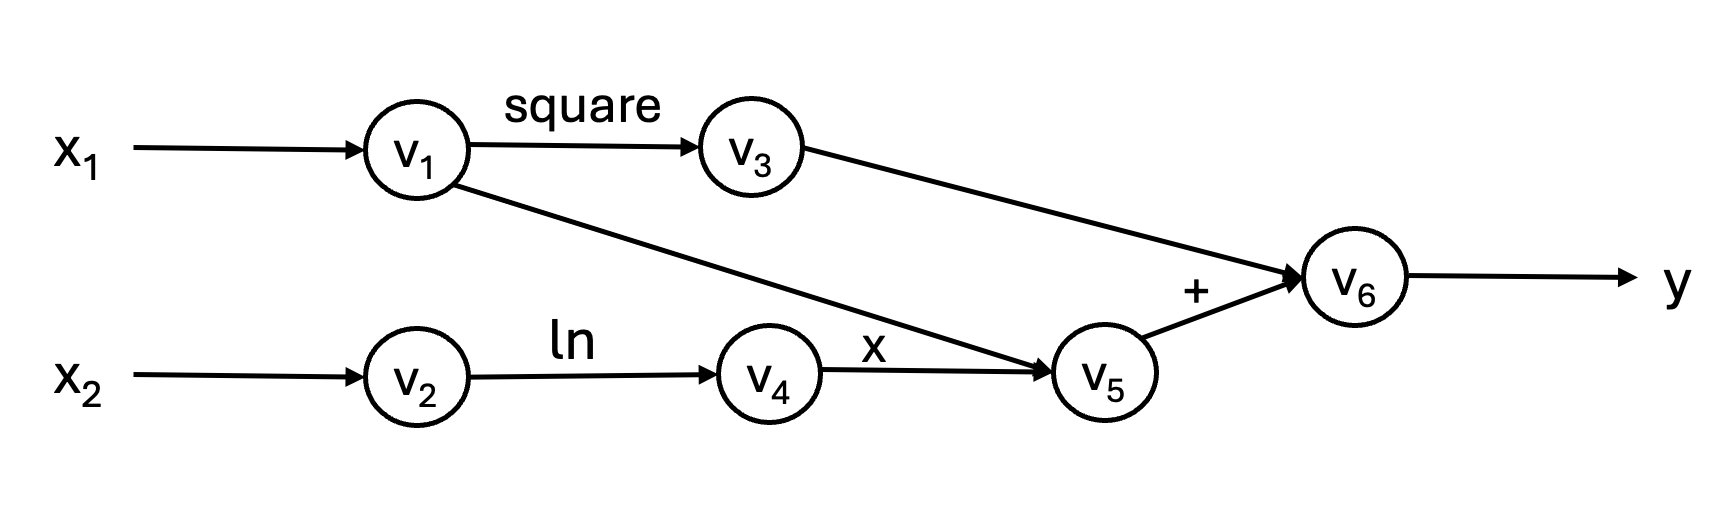
\includegraphics[width=0.7\textwidth]{Problem2.1.png}
\end{center}

\paragraph{2.2}
For the conputation graph in problem 2.1, substituting $x_1=2$ and $x_2=e$, we then have:
\begin{equation}
  \begin{split}
    f(x_1,x_2) &= x_1\cdot\ln(x_2)+x_1^2 \\
    &= 2\cdot\ln(e)+2^2 \\
    &= 2\cdot 1 + 4 \\
    &= 6
  \end{split}
\end{equation}
And the corresponding forward pass trace is:
\begin{equation}
\begin{split}
  v_1 &= x_1 = 2 \\
  v_2 &= x_2 = e \\
  v_3 &= x1^2 = 2^2 = 4 \\
  v_4 &= \ln(v_2) = \ln(e) = 1 \\
  v_5 &= v_1\times v_4 = 2\cdot 1 = 2 \\
  v_6 &=v_3 + v_5 = 2+ 4 = 6 \\
  y &= v_6 = 6
\end{split}
\end{equation}
The corresponding forward pass image is shown below:
\begin{center}
  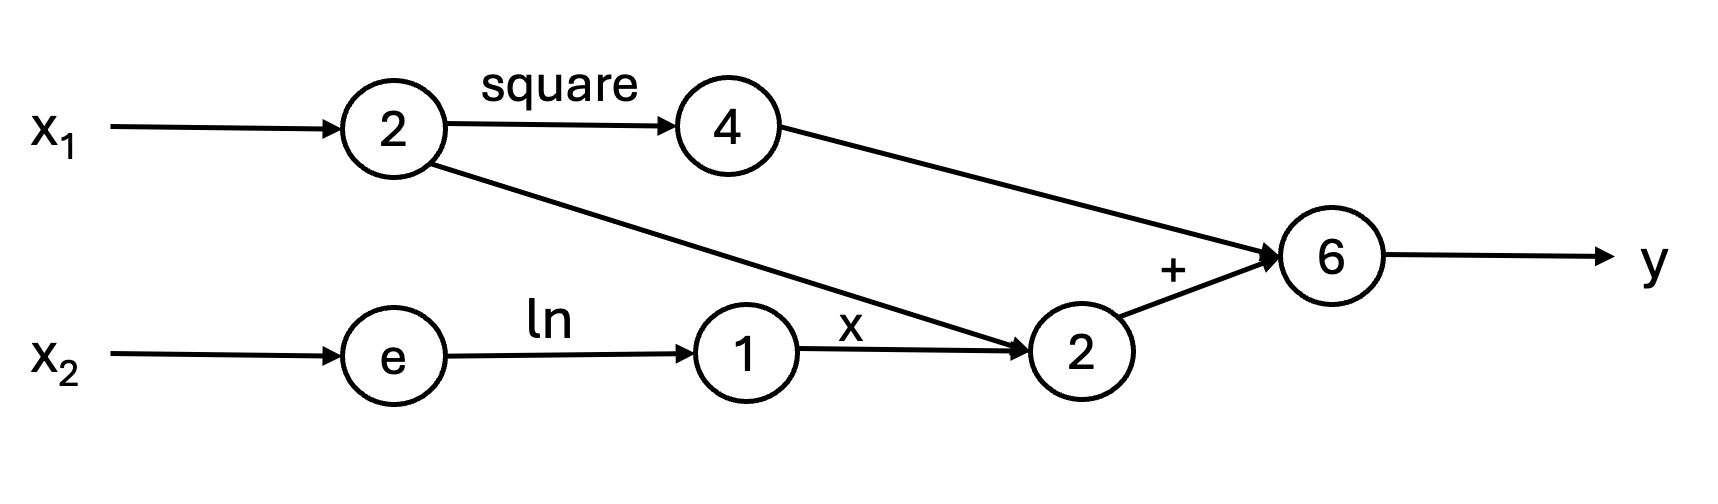
\includegraphics[width=0.7\textwidth]{Problem2.2.png}
\end{center}

\paragraph{2.3}
First, to calculate the derivate of the function with respect to $x_1$ with the forward-mode automatic differenta=iation, we can set its seed value to 1 and the seed value of $x_2$ to 0, and thus we have:
\begin{equation}
  \begin{split}
    \dot{v_1} &= 1 \\
    \dot{v_2} &= 0 \\
    \dot{v_3} &= 2\cdot v_1 \cdot \dot{v_1} = 2\cdot 2 \cdot 1 = 4 \\
    \dot{v_4} &= \frac{1}{v_2} \cdot \dot{v_2} = \frac{1}{e}\cdot 0 = 0 \\
    \dot{v_5} &= v_1\cdot \dot{v_4} + \ln(v_2)\cdot \dot{v_1} = 2\cdot 0 + 1\cdot 1 = 1 \\
    \dot{v_6} &= \dot{v_3} + \dot{v_5} = 4 + 1 = 5 \\
    \frac{\partial y}{\partial x_1} &= \dot{v_6} = 5
  \end{split}
\end{equation}
For the partial derivative of the function with respect to $x_2$, we can set its seed value to 1 and the seed value of $x_1$ to 0, and thus we have:
\begin{equation}
  \begin{split}
    \dot{v_1} &= 0 \\
    \dot{v_2} &= 1 \\
    \dot{v_3} &= 2\cdot v_1 \cdot \dot{v_1} = 2\cdot 2 \cdot 0 = 0 \\
    \dot{v_4} &= \frac{1}{v_2} \cdot \dot{v_2} = \frac{1}{e}\cdot 1 = \frac{1}{e} \\
    \dot{v_5} &= v_1\cdot \dot{v_4} + \ln(v_2)\cdot \dot{v_1} = 2\cdot\frac{1}{e} + 1\cdot 0 = \frac{2}{e} \\
    \dot{v_6} &= \dot{v_3} + \dot{v_5} = 0 + \frac{2}{e} = \frac{2}{e} \\
    \frac{\partial y}{\partial x_2} &= \dot{v_6} = \frac{2}{e}
  \end{split}
\end{equation}

\paragraph{2.4}
For the reverse-mode automatic differentiation, with $\overline{y} = \frac{\partial y}{\partial y} = 1$, we have:
\begin{equation}
  \begin{split}
    \overline{v_6} &= \overline{y} = 1 \\
    \overline{v_5} &= \overline{v_6} \frac{\partial v_6}{\partial v_5} = \overline{v_6} = 1 \\
    \overline{v_4} &= \overline{v_5} \frac{\partial v_5}{\partial v_4} = \overline{v_5} \cdot v_1 = 1\cdot 2 = 2 \\
    \overline{v_3} &= \overline{v_6} \frac{\partial v_6}{\partial v_3} = \overline{v_6} = 1 \\
    \overline{v_2} &= \overline{v_4} \frac{\partial v_4}{\partial v_2} = \overline{v_4} \cdot \frac{1}{v_2} = 2\cdot \frac{1}{e} = \frac{2}{e} \\
    \overline{v_1} &= \overline{v_5} \frac{\partial v_5}{\partial v_1} + \overline{v_3} \frac{\partial v_3}{\partial v_1} = \overline{v_5} + \overline{v_3} \cdot 2v_1 = 1 + 1\cdot 2\cdot 2 = 5 \\
  \end{split}
\end{equation}
Thus, the final value of the partial derivative of $y$ with respect to $x_1$ is:
\begin{equation}
  \frac{\partial y}{\partial x_1} = \overline{v_1} = 5
\end{equation}
For the partial derivative of $y$ with respect to $x_2$, we have:
\begin{equation}
  \frac{\partial y}{\partial x_2} = \overline{v_2} = \frac{2}{e}
\end{equation}

\end{document}